\documentclass[aspectratio=169]{beamer}
\setbeamercolor{background canvas}{bg=white}
\usetheme[numbering=fraction, progressbar=frametitle, block=fill]{metropolis}
\usepackage{appendixnumberbeamer}
\usepackage{tikz}
\usepackage{amsmath}
\usepackage{xcolor}
\usepackage{ifthen}
\usepackage{soul}
%%%%%%%%%%%%%%%%%%%%%%%%%%%%%%%%%%%%%%%%
%           Commandes perso            %
%%%%%%%%%%%%%%%%%%%%%%%%%%%%%%%%%%%%%%%%

%% Figures centrées, et en position 'here, top, bottom or page'
\newenvironment{figureth}{%
		\begin{figure}[htbp]
			\centering
	}{
		\end{figure}
		}


%% Tableaux centrés, et en position 'here, top, bottom or page'
\newenvironment{tableth}{%
		\begin{table}[htbp]
			\centering
			%\rowcolors{1}{coleurtableau}{coleurtableau}
	}{
		\end{table}
		}

%% Sous-figures centrées, en position 'top'
\newenvironment{subfigureth}[1]{%
	\begin{subfigure}[t]{#1}
	\centering
}{
	\end{subfigure}
}

\newcommand{\citationChap}[2]{%
	\epigraph{\og \textit{#1} \fg{}}{#2}
}

%% On commence par une page impaire quand on change le style de numérotation de pages
\let\oldpagenumbering\pagenumbering
\renewcommand{\pagenumbering}[1]{%
	\cleardoublepage
	\oldpagenumbering{#1}
}

%% Légende du dataset ISPRS
\newcommand\isprslegende{
Légende\,: \textcolor{Black}{blanc}\,: routes, \textcolor{Blue}{bleu}\,: bâtiments, \textcolor{Cerulean}{cyan}\,: végétation basse, \textcolor{OliveGreen}{vert}\,: arbres, \textcolor{Dandelion}{jaune}\,: véhicules, \textcolor{BrickRed}{rouge}\,: autre.
}

%% Dessiner des réseaux de neurones avec Tikz
\newcommand{\convlayer}[9]{%{h}{w}{d}{name}{color}{x}{y}{z}%{note w}{note h}{note d}
   \def\h{#1}
   \def\w{#2}
   \def\d{#3}
   \def\name{#4}
   \ifthenelse {\equal{#5} {}} {\def\col{white}} {\def\col{#5}}
   \def\x{#6}
   \ifthenelse {\equal{#7} {}} {\def\y{0}} {\def\y{#7}}
   \ifthenelse {\equal{#8} {}} {\def\z{0}} {\def\z{#8}}
   % ne faites pas ça chez vous !
   \ifthenelse {\equal{#9} {}} {\convlayercontinued{}{}{}} {\convlayercontinued#9}
}

\newcommand\convlayercontinued[3]{
   \def\notew{#1}
   \def\noteh{#2}
   \def\noted{#3}
   \coordinate (A) at (\x-\d/2,  \y-\h/2, \z-\w/2);
   \coordinate (B) at (\x-\d/2,  \y-\h/2, \z+\w/2);
   \coordinate (C) at (\x-\d/2,  \y+\h/2, \z+\w/2);
   \coordinate (D) at (\x-\d/2,  \y+\h/2, \z-\w/2);
   \coordinate (E) at (\x+\d/2,  \y-\h/2, \z-\w/2);
   \coordinate (F) at (\x+\d/2,  \y-\h/2, \z+\w/2);
   \coordinate (G) at (\x+\d/2,  \y+\h/2, \z+\w/2);
   \coordinate (H) at (\x+\d/2,  \y+\h/2, \z-\w/2);

    \draw [draw opacity=0.3, fill opacity=0.8, fill=\col!60!white] (A) -- (B) -- (C) -- (D) -- cycle;
    \draw [draw opacity=0.3, fill opacity=0.8, fill=\col!60!white] (A) -- (B) -- (F) -- (E) -- cycle;
    % Face haut
    %\draw [left color=\col!60!white, right color=\col!80!white, shading=axis, shading angle=180] (C) -- (D)  -- (H) -- (G) -- cycle;
    \draw [fill opacity=0.9, fill=\col!70!white] (C) -- node[rotate=45,above] {\small \name} (D) -- (H) -- (G) -- cycle;
    %\draw [fill opacity=0.9, fill=\col!70!white] (C) -- (D) -- node[above] {\small \name} (H) -- (G) -- cycle;
    % Face droite
    \draw [fill opacity=0.9, fill=\col!60!white] (E) -- node[pos=0.75,rotate=45,below] {\scriptsize \notew} (F) -- (G) --  (H) -- cycle;
    % Face avant
    %\draw [shading=axis, left color=\col!60!white, right color=\col!40!white, shading angle=-45] (B) -- node[above,rotate=90] {\scriptsize \noteh} (C) -- (G) -- (F) -- node[below] {\scriptsize \noted}  cycle;
    \draw [fill opacity=0.9, fill=\col!50!white] (B) -- node[above,rotate=90] {\scriptsize \noteh} (C) -- (G) -- (F) -- node[below] {\scriptsize \noted}  cycle;
}

\newcommand{\fclayer}[8]{%{h}{w}{name}{color}{x}{y}{z}
   \def\h{#1}
   \def\w{#2}
   \def\name{#3}
   \ifthenelse {\equal{#4} {}} {\def\col{white}} {\def\col{#4}}
   \def\x{#5}
   \def\y{#6}
   \def\z{#7}
   \def\note{#8}
   \coordinate (A) at (\x-\w/2,  \y-\h/2, \z);
   \coordinate (B) at (\x+\w/2,  \y-\h/2, \z);
   \coordinate (C) at (\x+\w/2,  \y+\h/2, \z);
   \coordinate (D) at (\x-\w/2,  \y+\h/2, \z);

   \pgfmathparse{4*\w}\let\boxwidth\pgfmathresult
    \draw [fill=\col] (A) -- node[below,text width=\boxwidth cm,align=center] {\scriptsize \note} (B) -- (C) -- (D) -- cycle;

    \node (N) at ($(A)!0.5!(B)+(0,-1,0)$) {\name};
}

\newcommand{\alexnet}[4]{%{scale}{x}{y}{z}
  \def\scale{#1}
  \def\alexx{#2}
  \def\alexy{#3}
  \def\alexz{#4}


  \def\coblue{blue!50!white}
  \def\fcgrey{gray!50!white}

  \convlayer{1.3*\scale}{1.3*\scale}{0.02*\scale}{Image}{\coblue}{\alexx}{\alexy}{\alexz}{{227}{227}{3}}
  \convlayer{1.1*\scale}{1.1*\scale}{0.08*\scale}{Conv1}{\coblue}{\alexx+0.7*\scale}{\alexy}{\alexz}{{55}{55}{96}}
  \convlayer{0.7*\scale}{0.7*\scale}{0.5*\scale}{Conv2}{\coblue}{\alexx+1.5*\scale}{\alexy}{\alexz}{{27}{27}{256}}
  \convlayer{0.5*\scale}{0.5*\scale}{0.8*\scale}{Conv3}{\coblue}{\alexx+2.6*\scale}{\alexy}{\alexz}{{13}{13}{384}}
  \convlayer{0.5*\scale}{0.5*\scale}{0.8*\scale}{Conv4}{\coblue}{\alexx+3.8*\scale}{\alexy}{\alexz}{{13}{13}{384}}
  \convlayer{0.5*\scale}{0.5*\scale}{0.5*\scale}{Conv5}{\coblue}{\alexx+4.8*\scale}{\alexy}{\alexz}{{13}{13}{256}}
  \fclayer{\scale}{0.1*\scale}{FC1}{\fcgrey}{\alexx+5.4*\scale}{\alexy}{\alexz}{4096}
  \fclayer{\scale}{0.1*\scale}{FC2}{\fcgrey}{\alexx+5.7*\scale}{\alexy}{\alexz}{4096}
  \fclayer{\scale}{0.1*\scale}{FC3}{\fcgrey}{\alexx+6.0*\scale}{\alexy}{\alexz}{1000}
}

\newcommand{\imagelayer}[7]{%{width}{x}{y}{z}{path}{text_up}{text_down}
    \pgfmathparse{#1}\let\w\pgfmathresult
    \begin{scope}[canvas is yz plane at x=#2]
     \node[transform shape] (source) at (#3, #4) {\includegraphics[angle=-90,width=\w cm]{#5}};
    \end{scope}
     \node [transform shape, rotate=45, above] at (source.east) {#6};
     \node [transform shape, rotate=45, below] at (source.west) {\scriptsize{#7}};
}

\def\fourier{\mathcal{F}}

\newcommand{\lightspectrum}{%
\pgfplotsset{
    % this *defines* a custom colormap ...
    colormap={slategraywhite}{color(0cm)=(red); color(1cm)=(red); color(2cm)=(red); color(3cm)=(red); color(4cm)=(orange); color(5cm)=(yellow); color(6cm)=(green); color(7cm)=(blue); color(8cm)=(blue); color(9cm)=(purple); color(10cm)=(purple); color(12cm)=(black)}
}
\node at (1.5, 2.7) {\small 1mm};
\node at (4, 3) {Infrarouge};
\node at (7.75, 2.7) {\small 800nm};
\node at (9, 3) {Visible};
\node at (10.5, 2.7) {\small 400nm};
\node at (12, 3) {Ultraviolet};
\node at (13.5, 2.7) {\small 10nm};
\draw[->] (1, 2.5) -- (14, 2.5);
\begin{axis}[hide axis,width=16cm,height=4cm,colormap name=slategraywhite]
\addplot[domain=20:1000,samples=1500,ultra thick, point meta=x*x,mesh]{sin(x*x/80)};
\end{axis}
}

% Union généralisée
\newcommand{\wbigcup}{\mathop{\bigcup}\displaylimits}

\newcommand{\res}[2]{%
	\ifthenelse{\isempty{#2}}%
	{\num{#1}}%
	{\num{#1}{\footnotesize $\pm$ \num{#2}}}}
\newcommand{\bres}[2]{%
	\ifthenelse{\isempty{#2}}%
	{\textbf{\num{#1}}}%
	{\textbf{\num{#1}}{\footnotesize $\pm$ \num{#2}}}}
\newcommand{\bbres}[2]{%
	\ifthenelse{\isempty{#2}}%
	{\textit{\num{#1}}}%
	{\textit{\num{#1}}{\footnotesize $\pm$ \num{#2}}}}

\newcommand{\drawkernel}[9]{
\begin{tikzpicture}
	\draw[step=1cm,gray!50!white,very thin] (0,0) grid (3,3);
	\kernelnode{0.5}{0.5}{#1};
	\kernelnode{0.5}{1.5}{#2};
	\kernelnode{0.5}{2.5}{#3};
	\kernelnode{1.5}{0.5}{#4};
	\kernelnode{1.5}{1.5}{#5};
	\kernelnode{1.5}{2.5}{#6};
	\kernelnode{2.5}{0.5}{#7};
	\kernelnode{2.5}{1.5}{#8};
	\kernelnode{2.5}{2.5}{#9};
\end{tikzpicture}
}

\newcommand{\kernelnode}[3]{%{x}{y}{value}
	\ifthenelse{\equal{#3}{0}}{
		\def\kcolor{gray}
	}{
		\def\kcolor{black}
	}
	\node[\kcolor] at (#1, #2) {#3};
}

\newcommand{\chapsummary}[1]{
\section*{Résumé du chapitre :}
\parbox{0.9\linewidth}{
\setlength{\parindent}{4ex}
#1}
}

\newcommand{\eqname}[1]{\tag*{\small (#1)}}

\usepackage{booktabs}
\usepackage[scale=2]{ccicons}
\usepackage{biblatex}
\addbibresource{demo.bib}
\usepackage{pgfplots}
\usepgfplotslibrary{dateplot}

\usepackage{xspace}
\newcommand{\themename}{\textbf{\textsc{metropolis}}\xspace}

\title{DEEP VISION IN ACTION}
\subtitle{From segmentation and detection to scene text understanding}
\date{\today}
\author{Duy V. Huynh, New AI Research (NAIR)}
\titlegraphic{\hfill
\includegraphics[height=1.5cm]{demo/figs/newai.png}}

\begin{document}

\maketitle

\begin{frame}{Outline}
  \setbeamertemplate{section in toc}[sections numbered]
  \tableofcontents[hideallsubsections]
\end{frame}

\begin{frame}
\begin{figure}
    \centering
    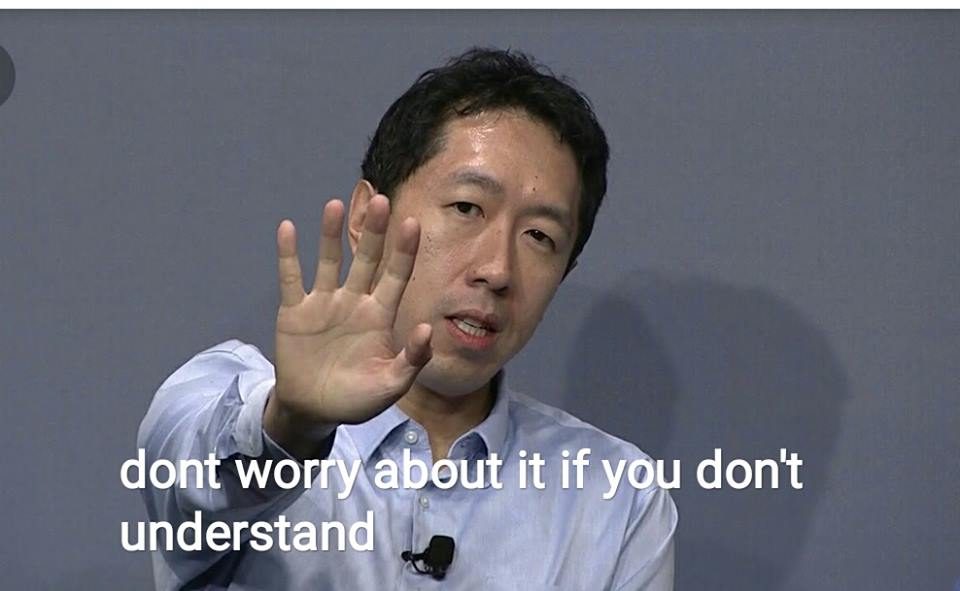
\includegraphics[scale=.4]{demo/figs/andrew.jpg}
\end{figure}
\end{frame}

\section{Recap: CNN backbone architecture}
\subsection{LeNet}
\begin{frame}{LeNet\footfullcite{Lecun98gradient-basedlearning}\footfullcite{Cun90handwrittendigit}
}
  \begin{columns}[T,c,onlytextwidth]
    \column{0.5\textwidth}
    \begin{itemize}
        \item Convolutional: locally connected, weight-sharing
        \item Subsampling
        \item Fully-connected layer
        \item Train by back-propagation
    \end{itemize}
    $\implies$ Basic components of modern ConvNets!
    \column{0.5\textwidth}
\begin{figure}
\resizebox{\textwidth}{!}{
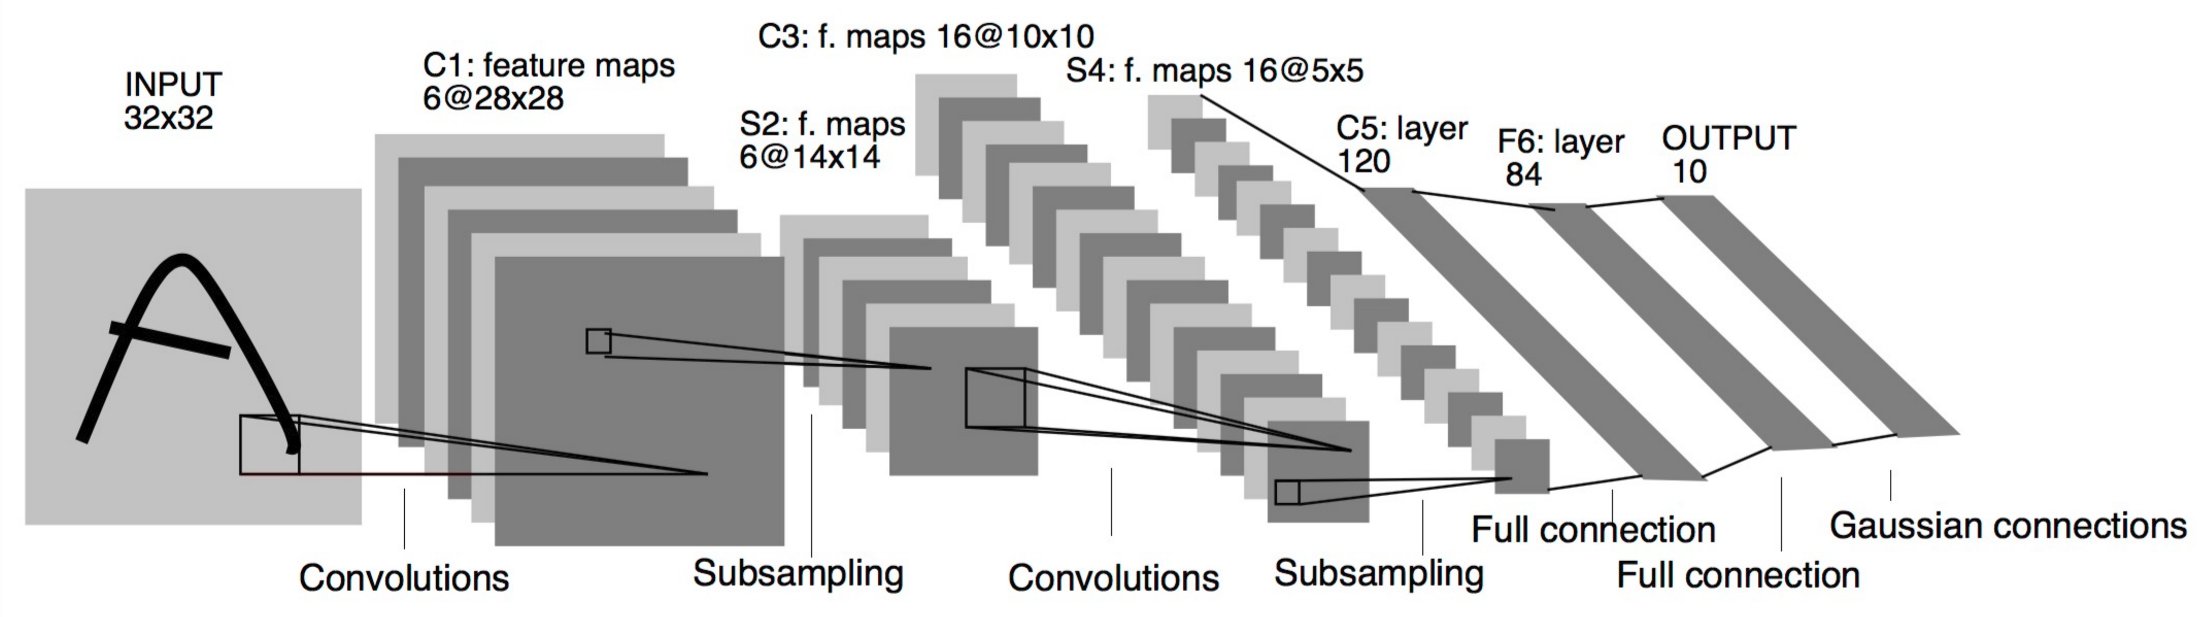
\includegraphics[scale=0.5]{demo/figs/lenet.png}
}
\caption{LeNet architecture}
\label{fig:lenet}
\end{figure}
  \end{columns}
\end{frame}

\subsection{AlexNet}

\begin{frame}{AlexNet\footfullcite{Krizhevsky_imagenetclassification}}
  \begin{columns}[T,c,onlytextwidth]
    \column{0.5\textwidth}
    \textcolor{red}{LeNet-style} backbone, and:
    \begin{itemize}
        \item \textcolor{red}{ReLU}\textsubscript{[Nair \& Hinton 2010]}
        \begin{itemize}
            \item Revolution of deep learning.
            \item Accelerate trainning, better than backprop + tanh.
        \end{itemize}
        \item \textcolor{red}{Dropout}\textsubscript{[Hinton et al 2012]}
        \begin{itemize}
            \item In-network ensembling.
            \item Reduce overfitting
        \end{itemize}
    \end{itemize}
    \column{0.5\textwidth}
\begin{figure}
\resizebox{\textwidth}{!}{
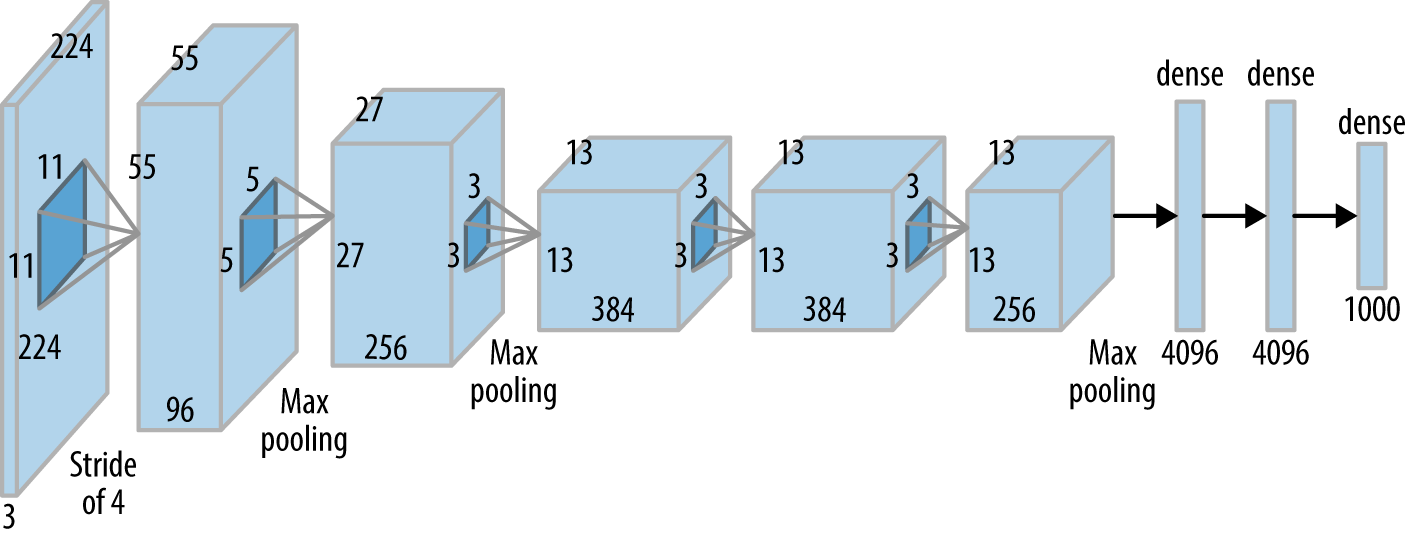
\includegraphics[scale=0.5]{demo/figs/alex.png}
}
\caption{AlexNet architecture}
\label{fig:alexnet}
\end{figure}
  \end{columns}

\end{frame}

\subsection{VGG}

\begin{frame}{VGG Net\footfullcite{Simonyan14verydeep}}
  \begin{columns}[T,c,onlytextwidth]
    \column{0.5\textwidth}
\begin{figure}
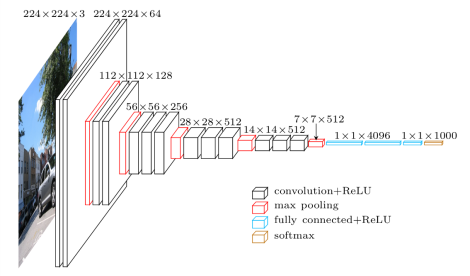
\includegraphics[scale=0.4]{demo/figs/vgg16.png}
\caption{VGG-16 architecture}
\label{fig:vgg16}
\end{figure}
\column{0.5\textwidth}
\textcolor{red}{Modularized} design:
\begin{itemize}
    \item 3x3 Conv = 1 module
    \item Stack the same module
    \item Same computation for each module (1/2 spatial size $\implies$ 2x filters)
\end{itemize}
\textcolor{red}{Stage-wise} trainning
\begin{itemize}
    \item VGG-11 $\implies$ VGG-13 $\implies$ VGG-16
\end{itemize}
\end{columns}
\end{frame}

\subsection{GoogleNet/Inception}
\begin{frame}{GoogleNet/Inception\footfullcite{Szegedy14goingdeeper}}
\begin{figure}
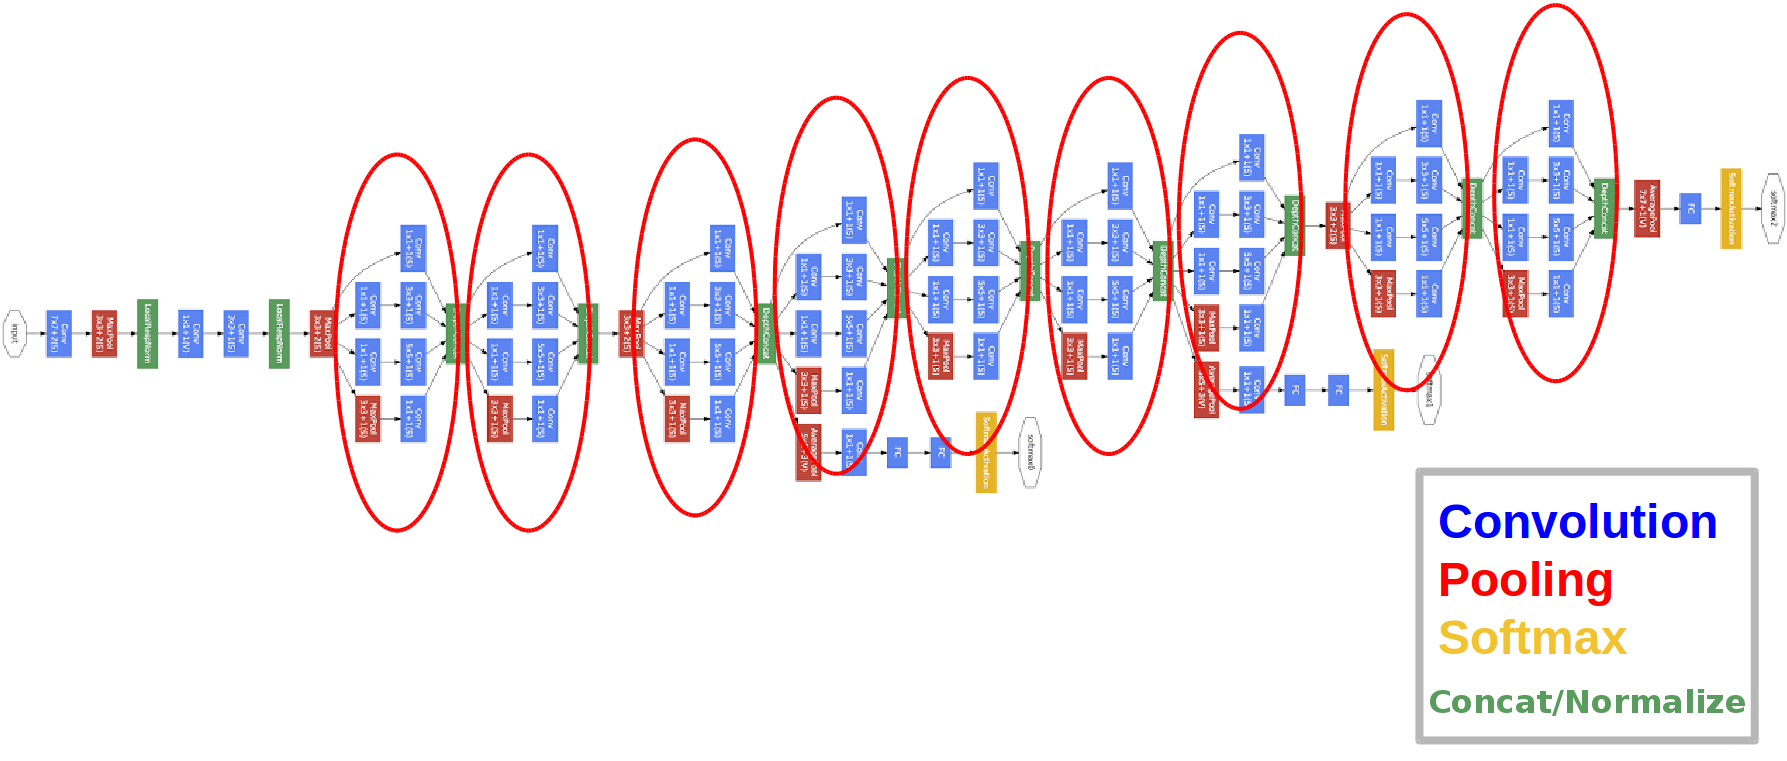
\includegraphics[scale=0.21]{demo/figs/inception.png}
\caption{GoogleNet/Inception architecture}
\label{fig:inception}
\end{figure}
\end{frame}

\begin{frame}{1$\times$1 convolution\footfullcite{minlin}}
  \begin{columns}[T,c,onlytextwidth]
    \column{0.5\textwidth}
\begin{figure}
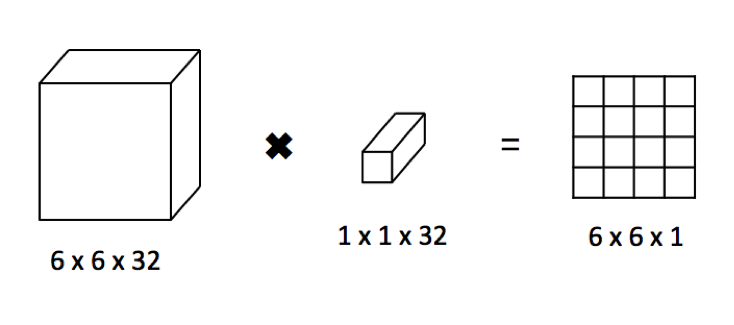
\includegraphics[scale=0.25]{demo/figs/1x1.png}
\caption{1x1 conv with 1 filter}
\label{fig:1x1}
\end{figure}
\column{0.5\textwidth}
\begin{figure}
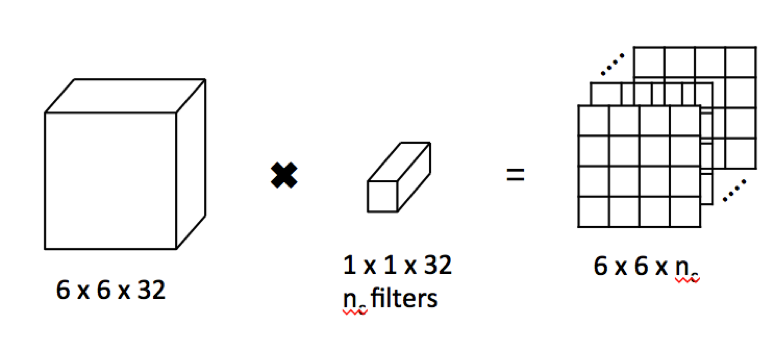
\includegraphics[scale=0.25]{demo/figs/1x1conv.png}
\caption{1x1 conv with n filter}
\label{fig:1x1conv}
\end{figure}

\end{columns}
\end{frame}

\begin{frame}{Why 1$\times$1 convolution?}
\begin{figure}
    \centering
    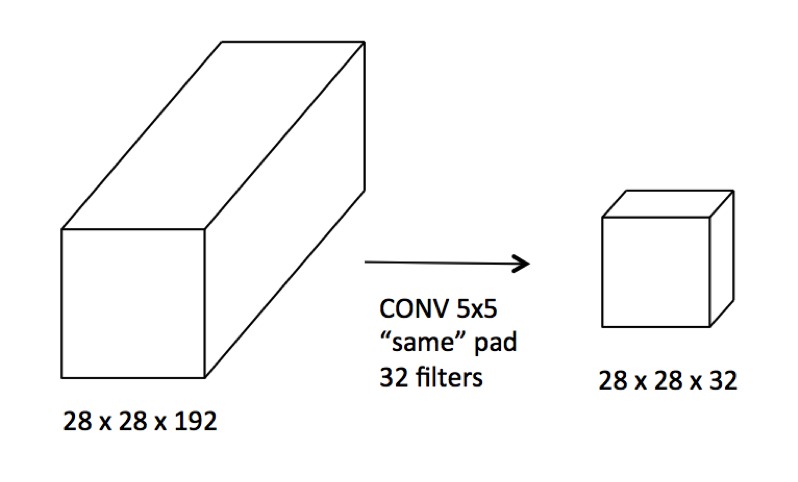
\includegraphics[scale=0.3]{demo/figs/cost1.png}
    \caption{5$\times$5 filter \times 32}
    \label{fig:cost1}
\end{figure}
$\implies$ Computational cost: $(28 \times 28 \times 32) \times (5 \times 5 \times 192) = 120.4M$
\end{frame}

\begin{frame}{Why 1$\times$1 convolution?}
\begin{figure}
    \centering
    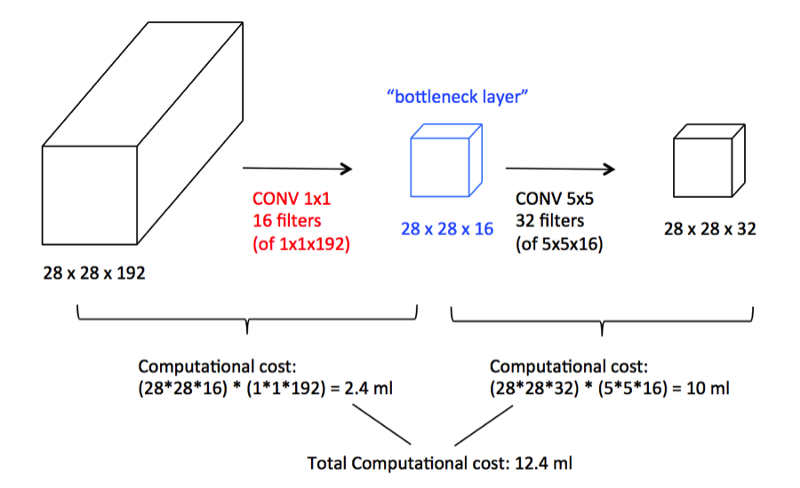
\includegraphics[scale=0.3]{demo/figs/cost2.png}
    \caption{"Bottleneck" transfer}
    \label{fig:cost2}
\end{figure}
$\implies$ 1$\times$1 reduces by nearly 10 times the total computational cost.

\end{frame}

\begin{frame}{Inception module}
\begin{figure}
    \centering
    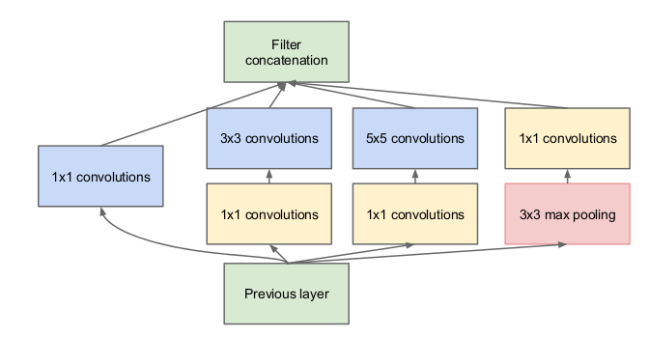
\includegraphics[scale=0.45]{demo/figs/inceptionmodule.png}
    \caption{Inception module}
    \label{fig:inceptionmodule}
\end{figure}
\end{frame}

\begin{frame}{GoogleNet/Inception\footfullcite{Szegedy14goingdeeper}}
\begin{figure}
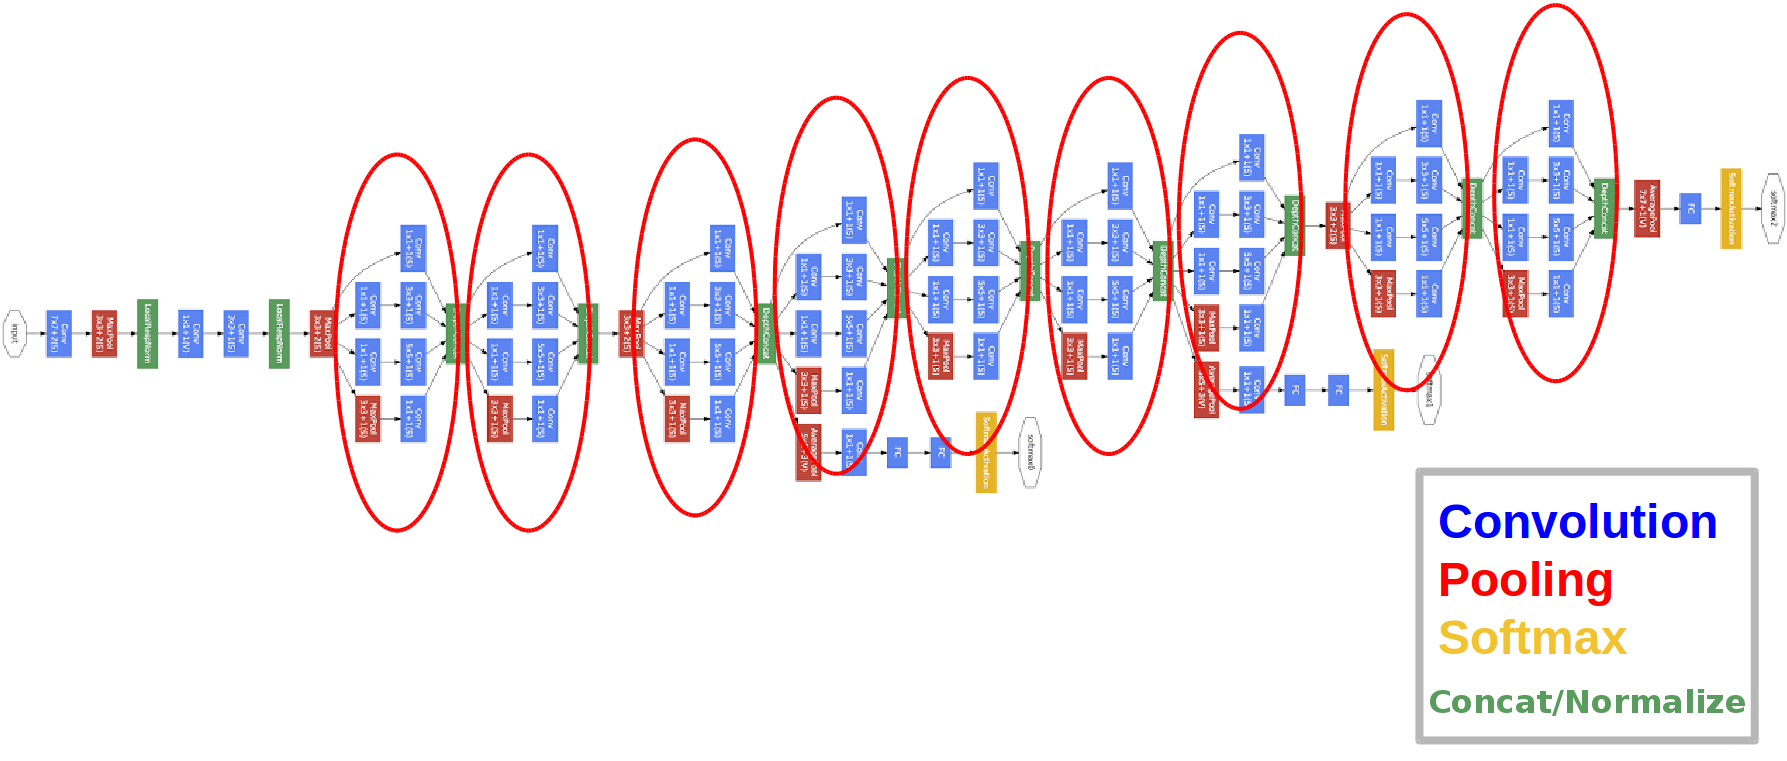
\includegraphics[scale=0.21]{demo/figs/inception.png}
\caption{GoogleNet/Inception architecture}
\label{fig:inception}
\end{figure}
\end{frame}

\begin{frame}{GooleNet/Inception\footfullcite{Szegedy14goingdeeper}}
\begin{alertblock}{Conclusions}
\begin{itemize}
    \item Multiple "branches"
    \begin{itemize}
        \item e.g., 1x1 conv, 3x3 conv, 5x5 conv, pool, ...
    \end{itemize}
    \item Shorcuts
    \begin{itemize}
        \item stand-alone 1x1, merged by concatenation method.
    \end{itemize}
    \item Bottlenek
    \begin{itemize}
        \item Reduce dimensionality by 1x1 conv.
    \end{itemize}
\end{itemize}
\end{alertblock}
\end{frame}

\subsection{ResNet}
\begin{frame}
\begin{center}
\begin{figure}
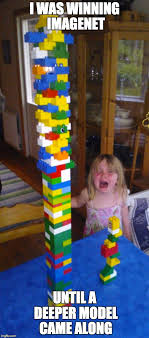
\includegraphics[scale=0.7]{demo/figs/meme.png}
\end{figure}
\end{center}
\end{frame}

\begin{frame}{Stacking more and more layers?\footfullcite{He2016DeepRL}}
\begin{figure}
    \centering
    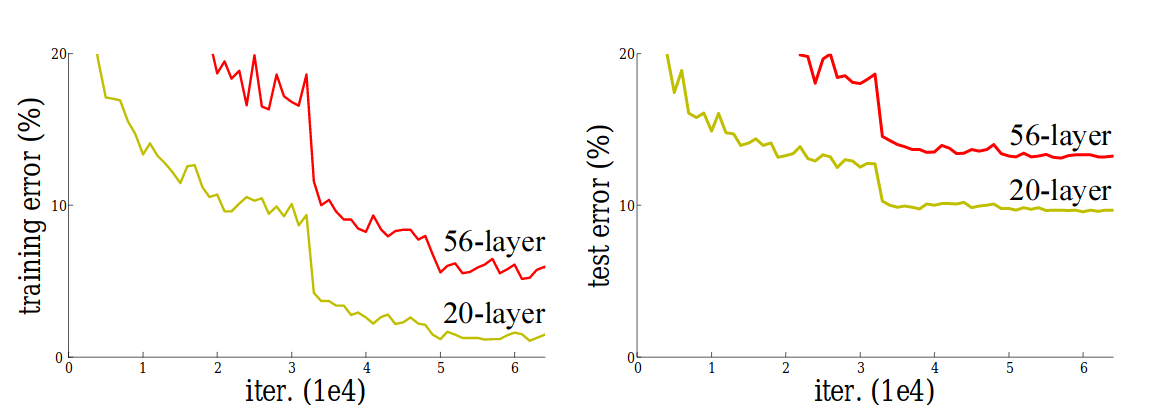
\includegraphics[scale = 0.2]{demo/figs/stacking.png}
    \caption{Training error (left) and test error (right) on CIFAR-10
with 20-layer and 56-layer “plain” networks}
    \label{fig:stacking}
\end{figure}    
\end{frame}

\begin{frame}{Deep residual learning\footfullcite{He2016DeepRL}}
\begin{columns}[T,c,onlytextwidth]
\column{0.5\textwidth}
\begin{figure}
    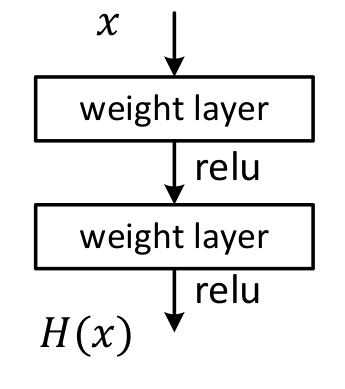
\includegraphics[scale=0.25]{demo/figs/plain.png}
    \caption{"Plain" connection in "plain" net}
    \label{fig:1x1}
\end{figure}

\column{0.5\textwidth}
\begin{alertblock}{}
$H(x)$ is any desired mapping, hope the small subnet fit $H(x)$.
\end{alertblock}
\end{columns}
\end{frame}

\begin{frame}{Deep residual learning\footfullcite{He2016DeepRL}}
\begin{columns}[T,c,onlytextwidth]
\column{0.5\textwidth}
\begin{figure}
    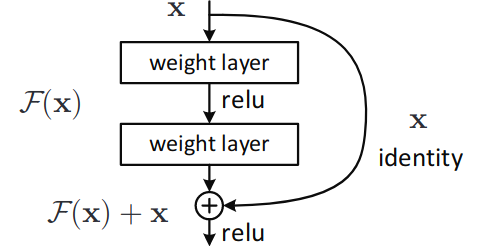
\includegraphics[scale=0.3]{demo/figs/residual.png}
    \caption{Residual connection in residual net}
    \label{fig:residual}
\end{figure}

\column{0.5\textwidth}
\begin{alertblock}{}
$H(x)$ is any desired mapping, \st{hope the small subnet fit $H(x)$} hope the small subnet fit $F(x)$ let $H(x) = F(x) + x$.
\begin{itemize}
    \item If identity were optimal, easy to set weights as 0.
    \item If optimal mapping is closer to identity, easier to find small fluctuations.
\end{itemize}
\end{alertblock}
\end{columns}
\end{frame}

\begin{frame}{ImageNet experiments}
\begin{figure}
    \centering
    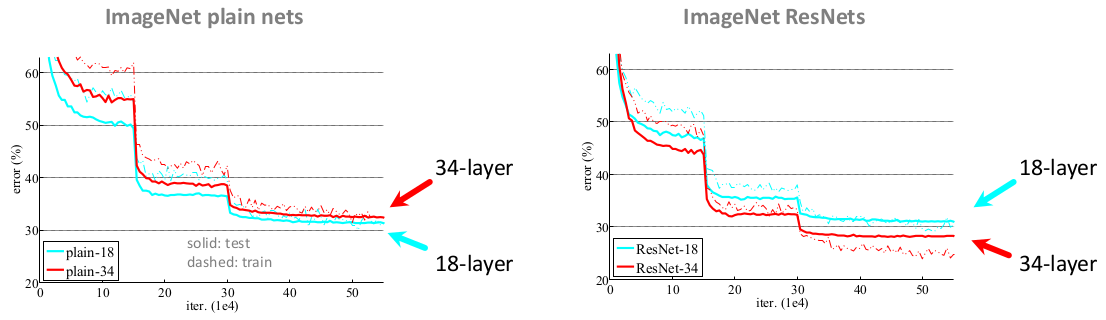
\includegraphics[scale=0.35]{demo/figs/imgnetex.png}
    \caption{Training on ImageNet}
    \label{fig:imgnetresnet}
\end{figure}

\begin{itemize}
    \item Deep ResNets can be trained without any difficulties.
    \item Deeper ResNets have lower trainning error, and also lower test error.
\end{itemize}
\end{frame}

\begin{frame}{ImageNet experiments}
\begin{figure}
    \centering
    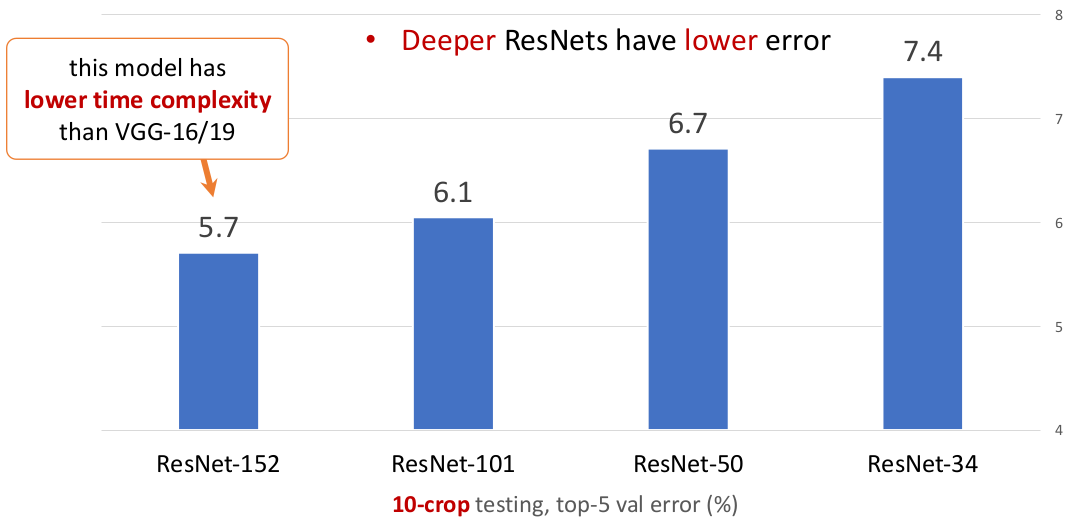
\includegraphics[scale=0.35]{demo/figs/ex2.png}
    \caption{Training more and more deeper model on ImageNet}
    \label{fig:imgnetresnet}
\end{figure}
\end{frame}

\begin{frame}{Residual connection beyond computer vision}
\begin{figure}
    \centering
    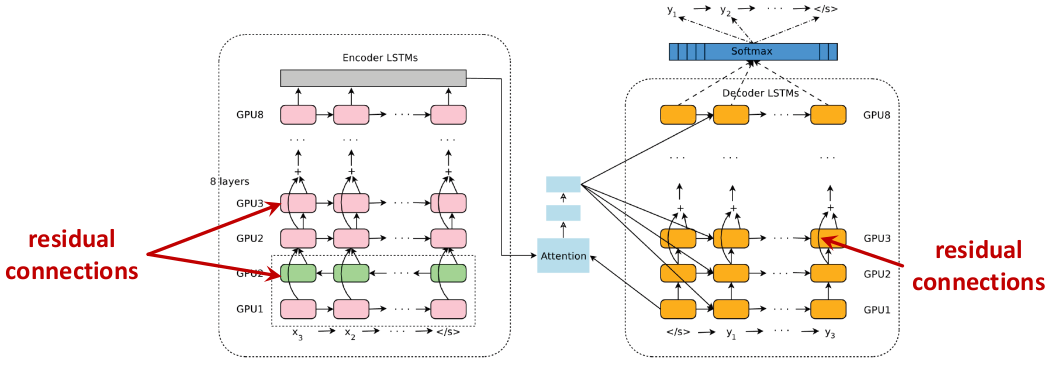
\includegraphics[scale=0.3]{demo/figs/nmt.png}
    \caption{Neural Machine Translation (NMT)\footfullcite{Wu2016GooglesNM}: 8-layer LSTM}
    \label{fig:nmt}
\end{figure}
\end{frame}

\begin{frame}{Residual connection beyond computer vision}
\begin{figure}
    \centering
    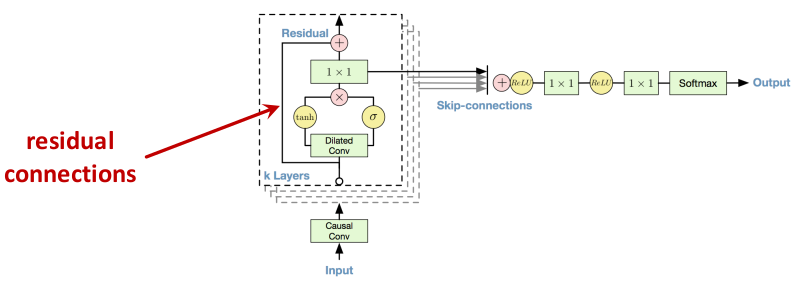
\includegraphics[scale=0.4]{demo/figs/wavenet.png}
    \caption{Speech synthesis (WaveNet)\footfullcite{Oord2016WaveNetAG}: Residual CNNs on 1-d sequence}
    \label{fig:wavenet}
\end{figure}
\end{frame}

\begin{frame}{Residual connection beyond computer vision}
\begin{figure}
    \centering
    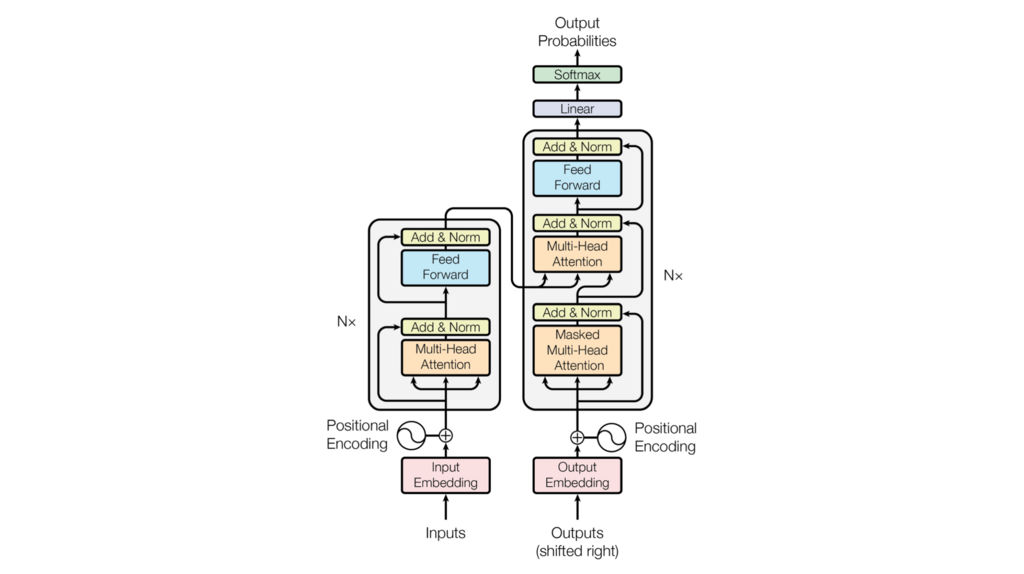
\includegraphics[scale=0.5]{demo/figs/transformer.png}
    \caption{Transformer\footfullcite{Vaswani2017AttentionIA}: }
    \label{fig:wavenet}
\end{figure}
\end{frame}

\begin{frame}{More architectures}
\begin{itemize}
    \item \textbf{Inception-ResNet}\textsubscript{[Szegedy et al 2017]}: Inception as transformation + residual connection.
    \item \textbf{DenseNet}\textsubscript{[Huang et al CVPR 2017]}: Densely connected shortcuts w/ concat.
    \item \textbf{Xception}\textsubscript{[Chollet CVPR 2017]}, \textbf{MobileNets}\textsubscript{[Howard et al 2017]}: DepthwiseConv
    \item \textbf{ShuffleNet}\textsubscript{[Zhang et al 2017]}: More group/DepthwiseConv + shuffle
    \item \textbf{ResNeXt}\textsubscript{[He et al CVPR 2017]}: Residual connection, multi branch, group-conv
    \item ...
\end{itemize}
\end{frame}

\section{Segmentation and Detection}
\begin{frame}{Computer Vision is not only Classification}
\begin{figure}
    \centering
    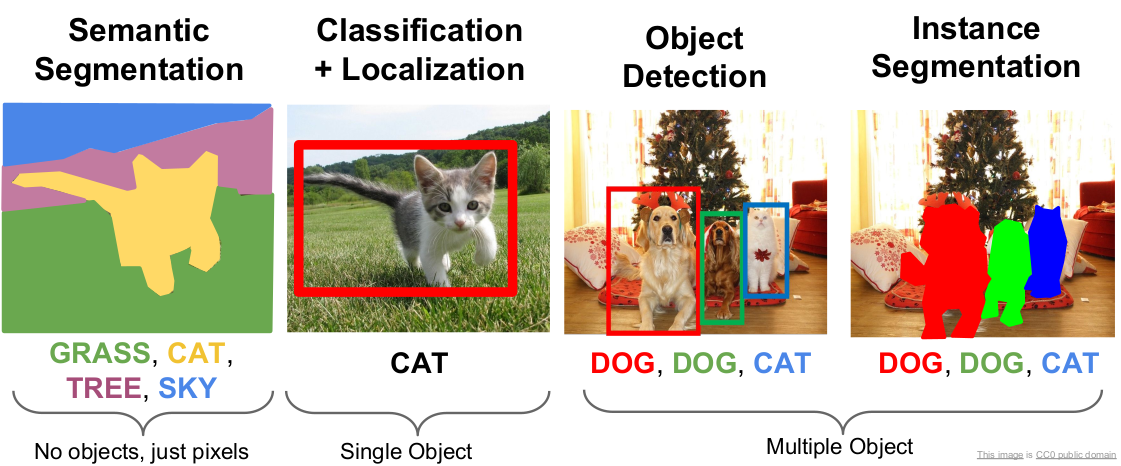
\includegraphics[scale=0.35]{demo/figs/cvtask.png}
\end{figure}
\end{frame}

\begin{frame}{Computer Vision is not only Classification}
\begin{figure}
    \centering
    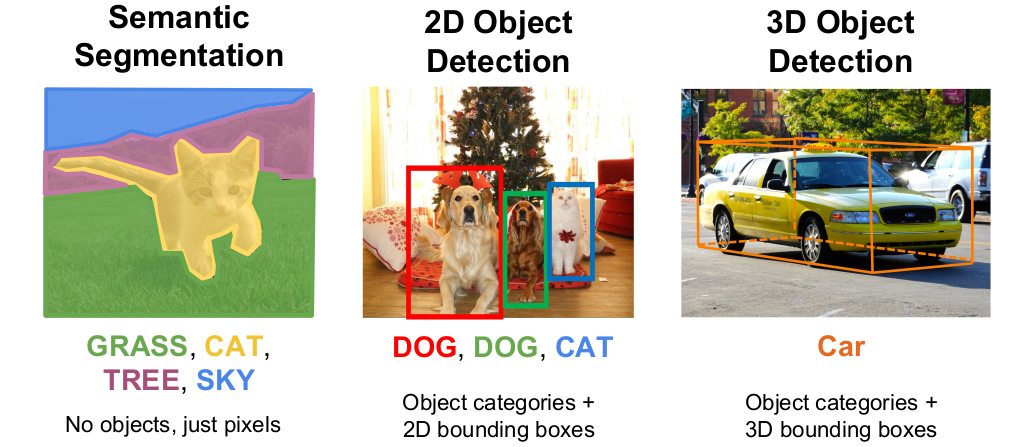
\includegraphics[scale=0.35]{demo/figs/cvtask2.png}
\end{figure}
\end{frame}

\begin{frame}{Semantic Segmentation}
\begin{columns}[T,c,onlytextwidth]
\column{0.5\textwidth}
\begin{center}
\centering
\begin{itemize}
    \item Label each pixel in the image with a category label.
    \item Don't differentiate instances, only care about pixels.
\end{itemize}
\end{center}
\column{0.5\textwidth}
\begin{figure}
    \centering
    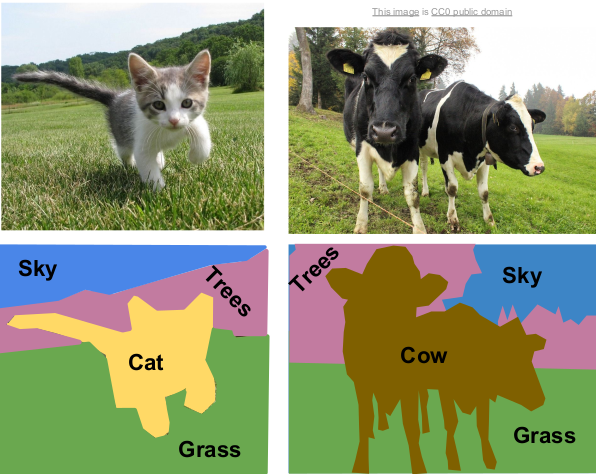
\includegraphics[scale=0.3]{demo/figs/sematicseg.png}
\end{figure}
\end{columns}
\end{frame}

\begin{frame}{Semantic Segmentation Idea: Sliding Window}
\begin{figure}
    \centering
    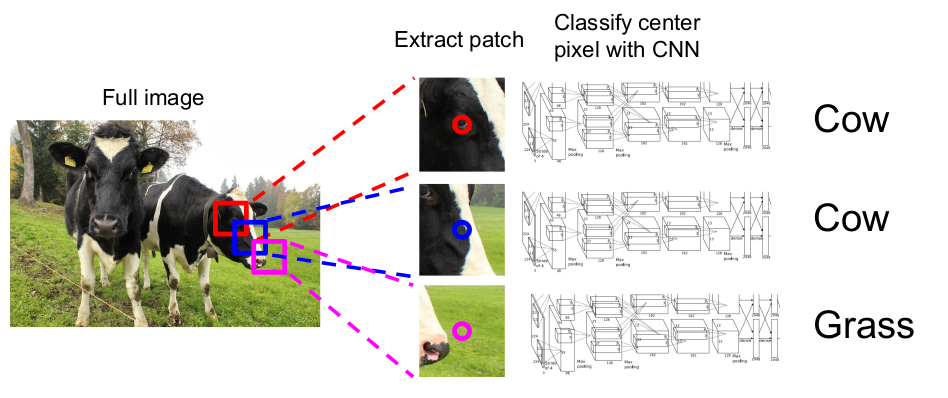
\includegraphics[scale=0.35]{demo/figs/sw.png}
\end{figure}
$\implies$ \textbf{Problem}: Computational cost is very expensive! Not reusing shared features between overlapping patches.
\end{frame}

\begin{frame}{Semantic Segmentation Idea: Fully Convolutional}
\begin{figure}
    \centering
    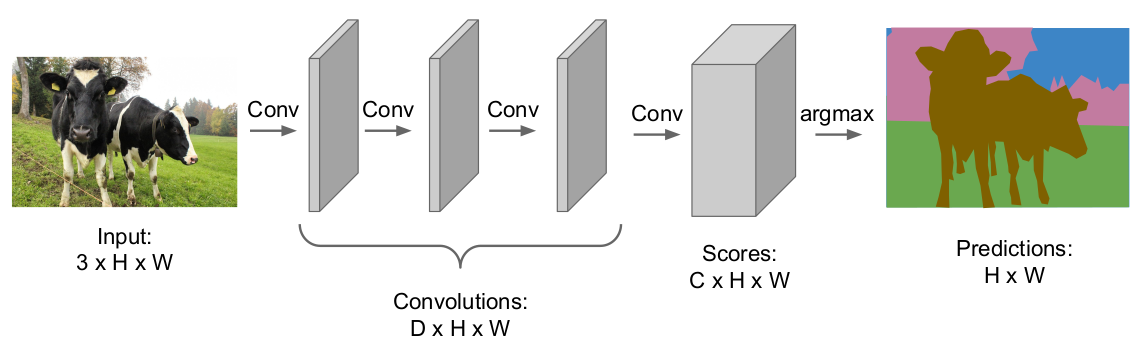
\includegraphics[scale=.3]{demo/figs/fconv.png}
\end{figure}
\begin{itemize}
    \item Make predictions for \textcolor{red}{all pixels at once}
\end{itemize}
$\implies$ \textbf{Problem} again: Convolutions at original image resolution is still very expensive.
\end{frame}

\begin{frame}{Semantic Segmentation Idea: Fully Convolutional}
 \begin{figure}
    \centering
    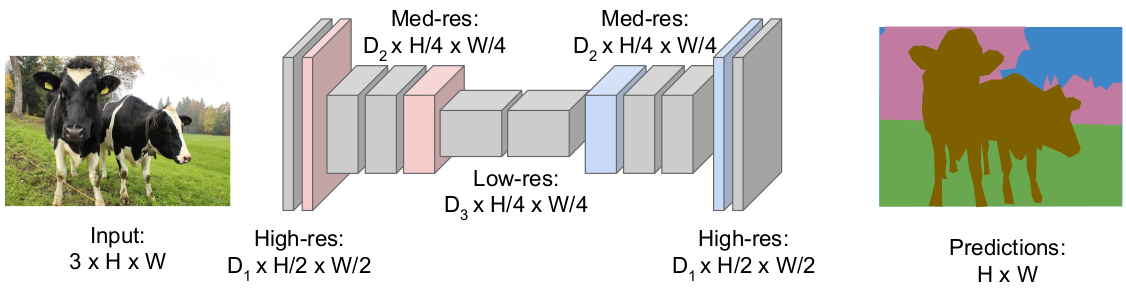
\includegraphics[scale=.35]{demo/figs/fconv2.png}
    \caption{Fully Convolutional Networks for Semantic Segmentation}
\end{figure}  
\end{frame}

\begin{frame}{Semantic Segmentation Idea: Fully Convolutional}
\begin{figure}
    \centering
    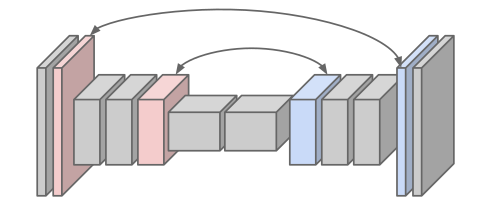
\includegraphics[scale=.25]{demo/figs/encoderdecoder.png}
\end{figure}
\begin{itemize}
    \item Design network as a bunch of convolutional layers, with \textbf{down-sampling} and \textbf{up-sampling} inside\footfullcite{Shelhamer2015FullyCN}.
    \item \textcolor{red}{Down-sampling}: Pooling, strided convolution $\implies$ \textcolor{blue}{Up-sampling, Un-pooling ???}
\end{itemize}
\end{frame}

\begin{frame}{Naive Idea for Up-sampling}
\begin{center}
    \begin{figure}
    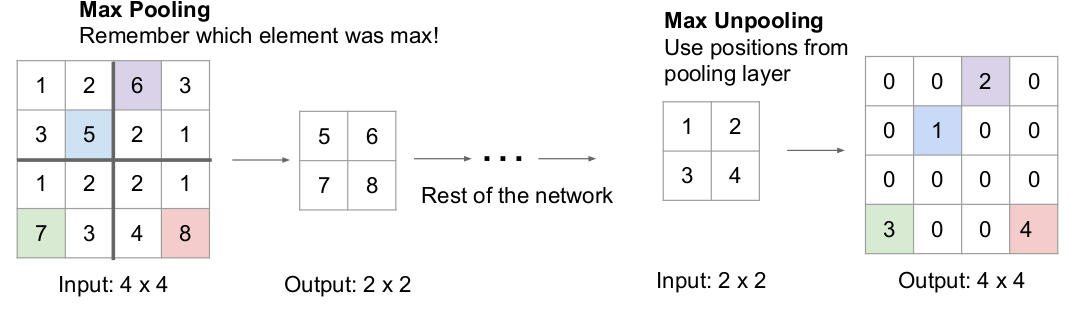
\includegraphics[scale=.35]{demo/figs/unpool1.png}
\end{figure}
\end{center}
\end{frame}

\begin{frame}{Naive Idea for Up-sampling}
\begin{center}
    \begin{figure}
    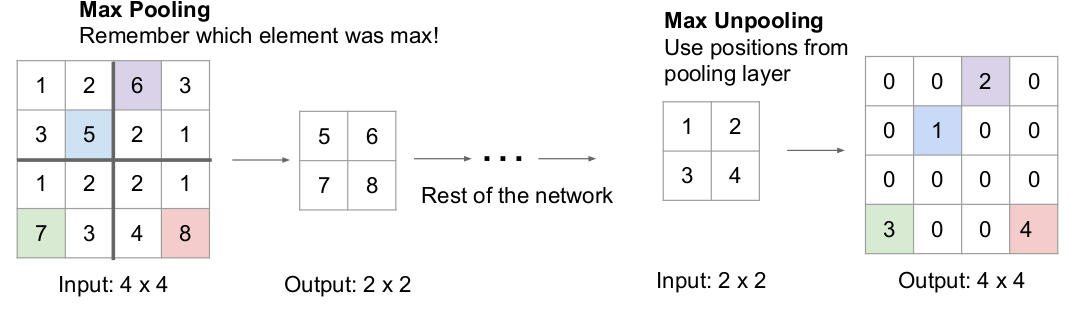
\includegraphics[scale=.35]{demo/figs/unpool1.png}
\end{figure}
\end{center}
\begin{itemize}
    \item \textcolor{red}{Nonlearnable}
$\implies$ Not a very good idea. 
\end{itemize}
\end{frame}

\begin{frame}{Learnable Up-sampling: Transpose Convolution}
\begin{figure}
    \centering
    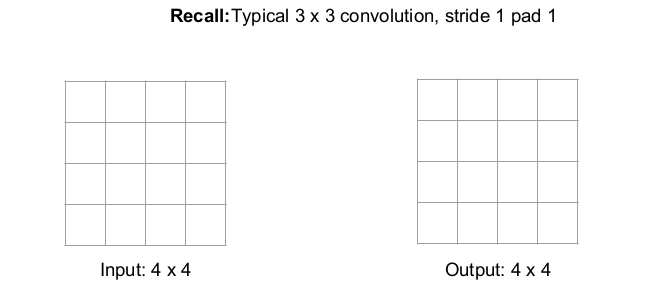
\includegraphics[scale=.4]{demo/figs/tconv1.png}
\end{figure}
\end{frame}

\begin{frame}{Learnable Up-sampling: Transpose Convolution}
\begin{figure}
    \centering
    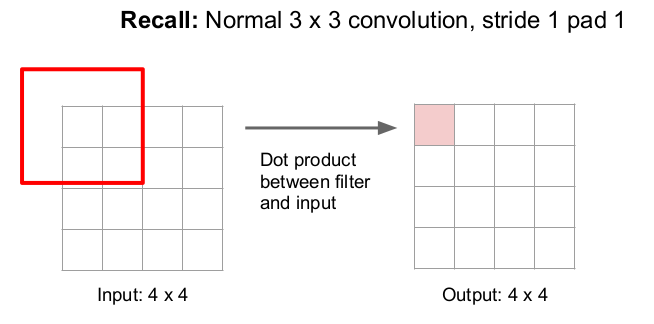
\includegraphics[scale=.4]{demo/figs/tconv2.png}
\end{figure}
\end{frame}

\begin{frame}{Learnable Up-sampling: Transpose Convolution}
\begin{figure}
    \centering
    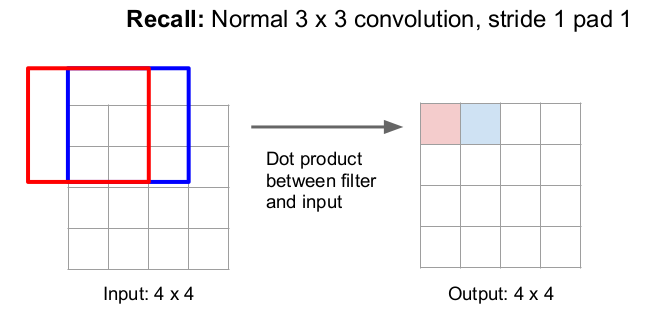
\includegraphics[scale=.4]{demo/figs/tconv3.png}
\end{figure}
\end{frame}

\begin{frame}{Learnable Up-sampling: Transpose Convolution}
\begin{figure}
    \centering
    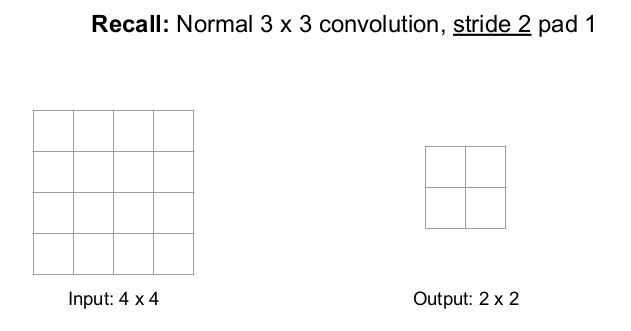
\includegraphics[scale=.4]{demo/figs/tconv4.png}
\end{figure}
\end{frame}

\begin{frame}{Learnable Up-sampling: Transpose Convolution}
\begin{figure}
    \centering
    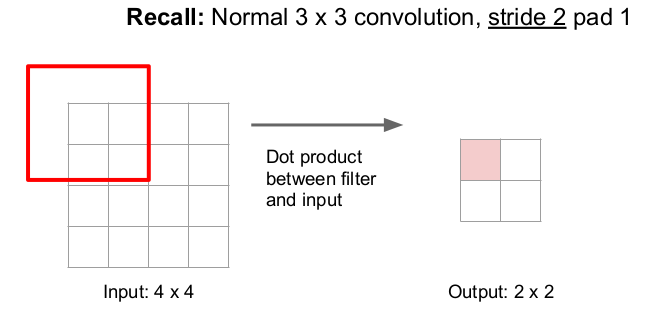
\includegraphics[scale=.4]{demo/figs/tconv5.png}
\end{figure}
\end{frame}

\begin{frame}{Learnable Up-sampling: Transpose Convolution}
\begin{figure}
    \centering
    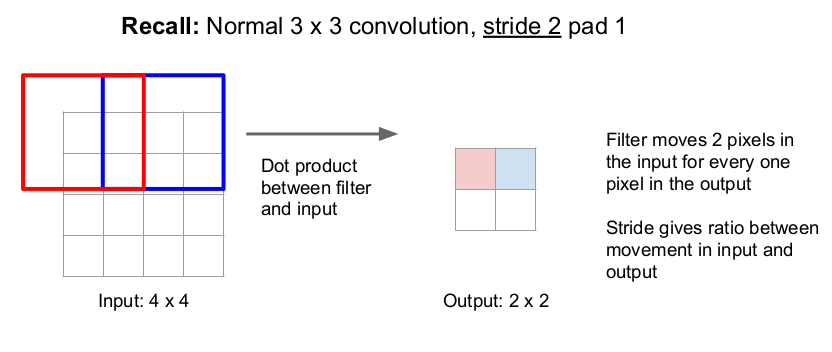
\includegraphics[scale=.4]{demo/figs/tconv6.png}
\end{figure}
\end{frame}

\begin{frame}{Learnable Up-sampling: Transpose Convolution}
\begin{figure}
    \centering
    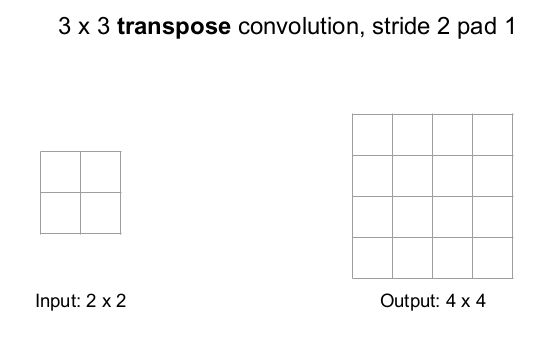
\includegraphics[scale=.4]{demo/figs/tconv7.png}
\end{figure}
\end{frame}

\begin{frame}{Learnable Up-sampling: Transpose Convolution}
\begin{figure}
    \centering
    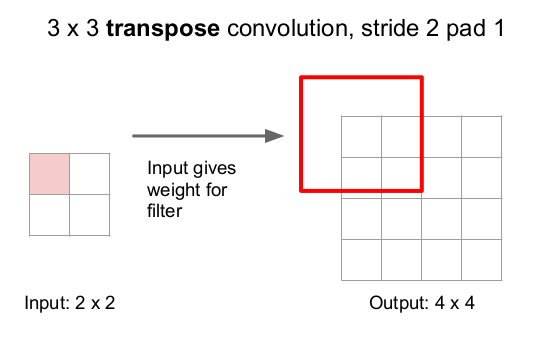
\includegraphics[scale=.4]{demo/figs/tconv8.png}
\end{figure}
\end{frame}

\begin{frame}{Learnable Up-sampling: Transpose Convolution}
\begin{figure}
    \centering
    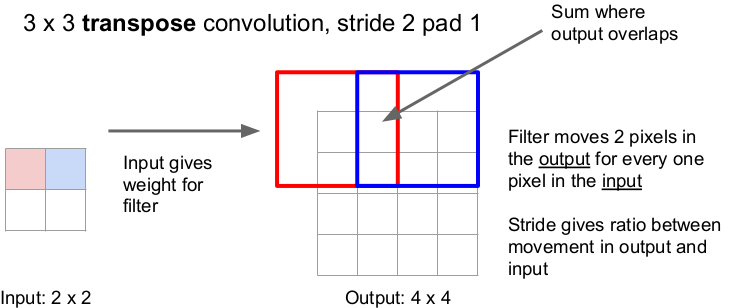
\includegraphics[scale=.4]{demo/figs/tconv11.png}
\end{figure}
$\implies$ Transpose convolution a.k.a. Deconvolution, Upconvolution, Fractionally strided convolution, Backward convolution, ..
\end{frame}

\begin{frame}{Learnable Up-sampling: 1D Example}
\begin{figure}
    \centering
    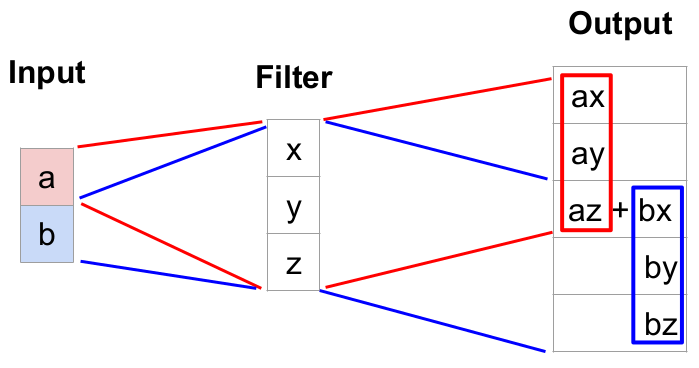
\includegraphics[scale=.35]{demo/figs/tconv12.png}
\end{figure}
\begin{itemize}
    \item Output contains copies of the filter weighted by the input, summing at where at overlaps in the output.
    \item Need to crop one pixel from output to make output exactly 2x input.
\end{itemize}
\end{frame}

\begin{frame}{Semantic Segmentation Idea: Fully Convolutional}
\begin{figure}
    \centering
    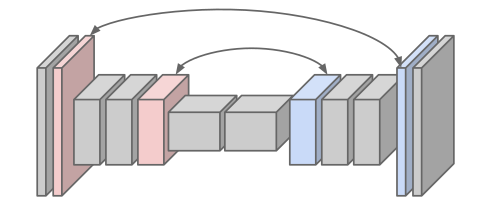
\includegraphics[scale=.25]{demo/figs/encoderdecoder.png}
\end{figure}
\begin{itemize}
    \item Design network as a bunch of convolutional layers, with \textbf{down-sampling} and \textbf{up-sampling} inside\footfullcite{Shelhamer2015FullyCN}.
    \item \textcolor{red}{Down-sampling}: Pooling, strided convolution $\implies$ \textcolor{blue}{Up-sampling: Un-pooling, strided transpose convolution}
\end{itemize}
\end{frame}

\begin{frame}{Classification and Localization}
\begin{figure}
    \centering
    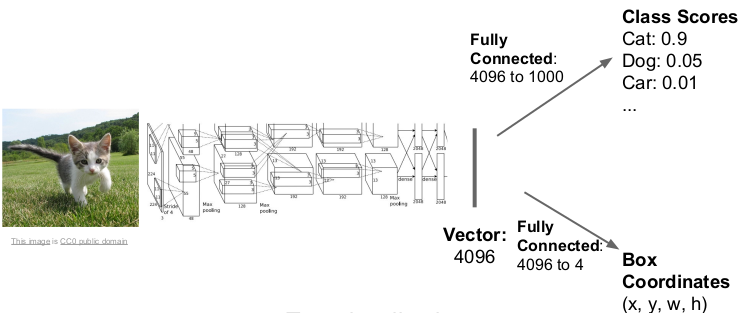
\includegraphics[scale=0.4]{demo/figs/object.png}
    \caption{Single Object Detection}
\end{figure}
\end{frame}

\begin{frame}{Classification and Localization}
How would we train such a single object detection network that produces 4 + n values?
\begin{itemize}
    \item Predicting the class of the object (n class probabilities) is a \textcolor{red}{classification} problem.
    \item Predicting the four coordinates for the bounding box is a \textcolor{red}{regression} problem.
\end{itemize}
$\implies$ Need a loss function that combines these two problems.
\end{frame}

\begin{frame}{Classification and Localization}
\begin{itemize}
    \item \textcolor{red}{Localization loss}
    
    $\mathcal{L}_{loc} = \sum_{i = 1}^{4}\left | x_{pred, i} - x_{truth, i} \right |$
    
    \item \textcolor{red}{Confidence loss}
    
    $\mathcal{L}_{conf} = \frac{-1}{N} (\sum_{i = 1}^{N} y_{truth, i} \cdot log(y_{pred, i}))$
    
\end{itemize}
$\implies$ \textcolor{red}{Combined loss function}

\centering

$\mathcal{L} = \mathcal{L}_{loc} + \alpha \cdot \mathcal{L}_{conf}$

\end{frame}

\begin{frame}{Classification and Localization}
\begin{figure}
    \centering
    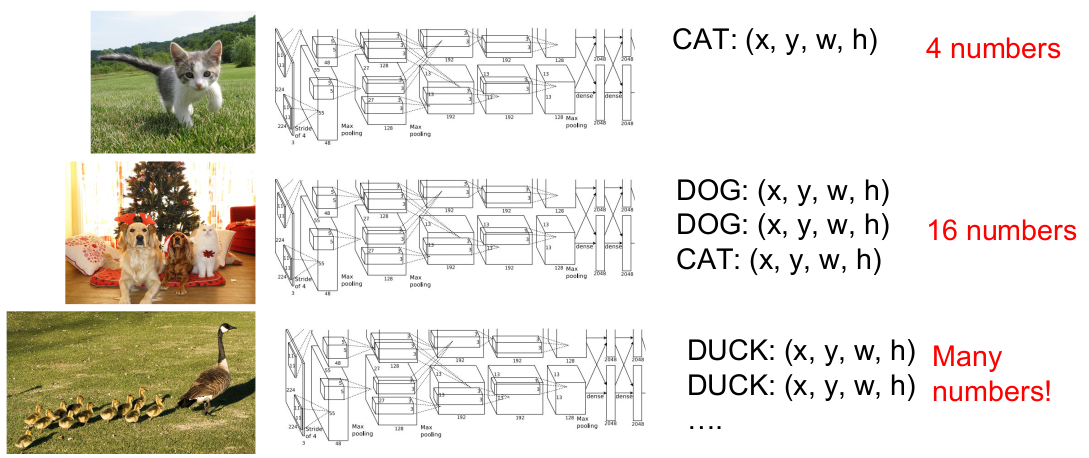
\includegraphics[scale=.35]{demo/figs/ob2.png}
\end{figure}
\end{frame}

\subsection{Region proposal methods}
% R-CNN, Fast R-CNN, Faster R-CNN, Mask R-CNN

\begin{frame}{Multiple Object Detection: Region Proposal Methods}
\begin{figure}
    \centering
    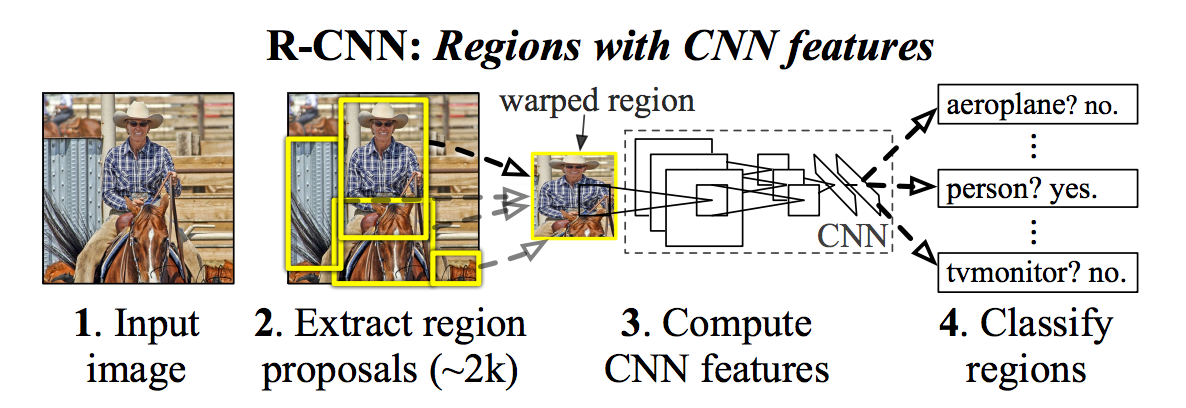
\includegraphics[scale=.3]{demo/figs/rcnn.png}
    \caption{Region Convolutional Neural Network\footfullcite{girshick2014rcnn}}
\end{figure}
\end{frame}

\begin{frame}{Multiple Object Detection: Region Proposal Methods}
\begin{alertblock}{Problems with R-CNN}

\begin{itemize}
    \item Extracting 2,000 regions for each image based on selective search.
    \item Extracting features using CNN for every image region. Suppose we have N images, then the number of CNN features will be N $\times$ 2,000.
    \item The entire process of object detection using R-CNN has three models: 
    \begin{itemize}
        \item CNN for feature extraction.
        \item Linear SVM classifier for identifying objects.
        \item Regression model for tightening the bounding boxes.
    \end{itemize}
\end{itemize}
\end{alertblock}

$\implies$ \textcolor{red}{Very slow}, it takes around 40-50 seconds to make predictions for each image.
\end{frame}

\begin{frame}{Multiple Object Detection: Region Proposal Methods}
\begin{figure}
    \centering
    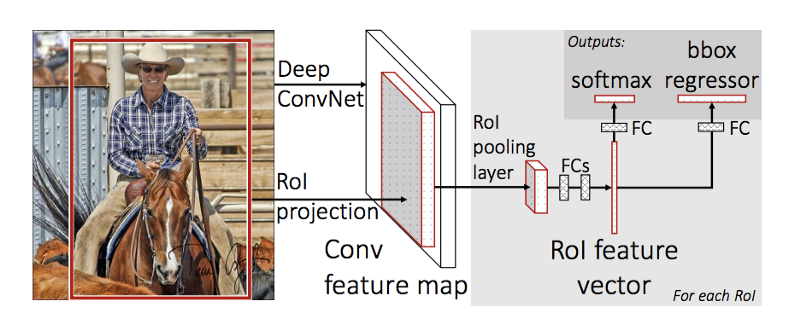
\includegraphics[scale=.4]{demo/fastrcnn.png}
    \caption{Fast R-CNN\footfullcite{Girshick2015FastR}}
\end{figure}
\end{frame}

\begin{frame}{Multiple Object Detection: Region Proposal Methods}

$\implies$ Still have a \textcolor{red}{problem}, it also uses selective search as a proposal method to find the Regions of Interest, which is a slow and time consuming process. It takes around 2 seconds per image to detect objects, which is much better compared to RCNN
\end{frame}


\begin{frame}{Multiple Object Detection: Region Proposal Methods}
\begin{columns}[T,c,onlytextwidth]
\column{0.5\textwidth}
\begin{figure}
\resizebox{\textwidth}{!}{
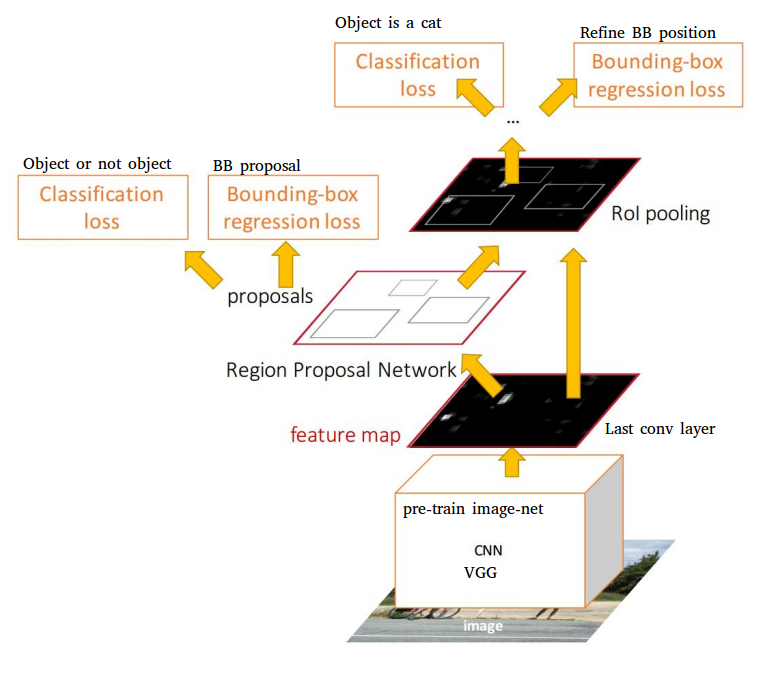
\includegraphics[scale=0.16]{demo/figs/ob4.png}
}
\caption{Faster R-CNN}
\end{figure}
\column{0.5\textwidth}
Insert \textcolor{red}{Region Proposal Network (RPN)} to predict proposals from features. Jointly train with 4 losses:
\begin{itemize}
    \item RPN classify object/not object
    \item RPN regress box coordinates
    \item Final classification score (object classes)
    \item Final box coordinates
\end{itemize}
  \end{columns}
  
\end{frame}

\begin{frame}{Multiple Object Detection: Region Proposal Methods}
\begin{figure}
    \centering
    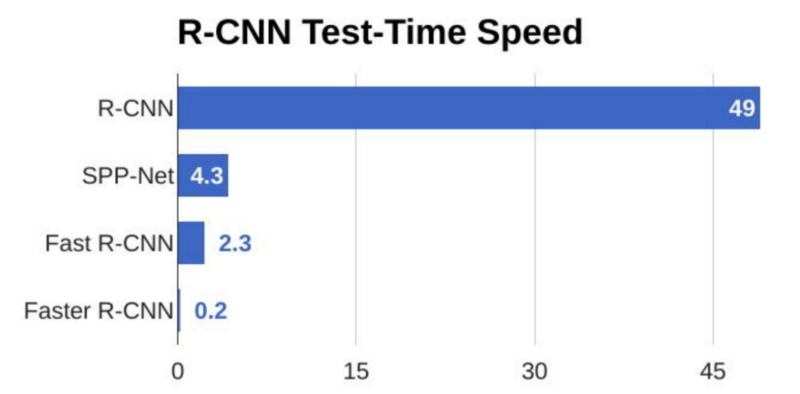
\includegraphics[scale=.3]{demo/figs/ex.png}
    \caption{Experimentation results}
\end{figure}
\end{frame}

\begin{frame}{Instance Segmentation}
\begin{figure}
    \centering
    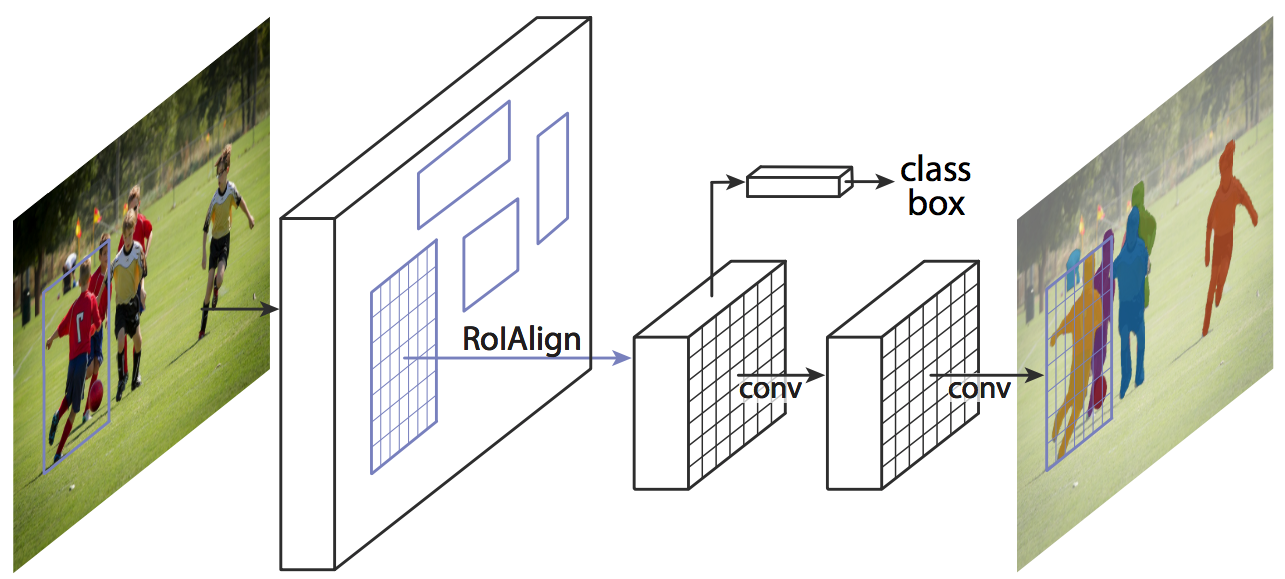
\includegraphics[scale=.2]{demo/figs/mask.png}
    \caption{Mask R-CNN\footfullcite{He2017MaskR}}
\end{figure}
\end{frame}

\begin{frame}{Instance Segmentation}
\begin{figure}
    \centering
    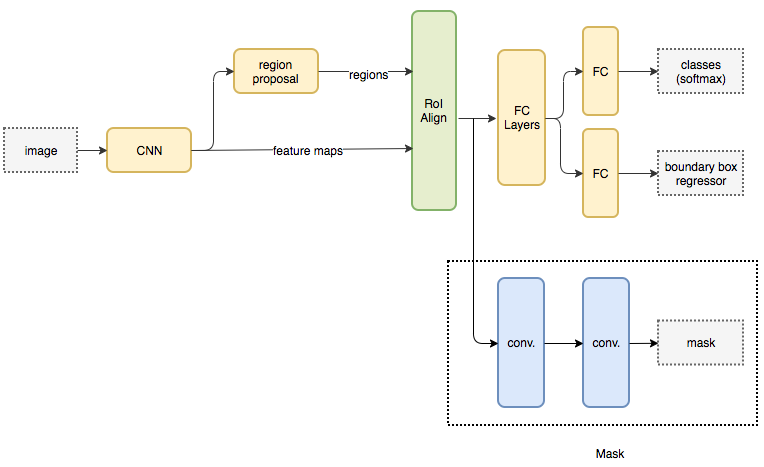
\includegraphics[scale=.35]{demo/figs/mask2.png}
    \caption{Mask R-CNN architecture}
\end{figure}
\end{frame}

\begin{frame}{Instance Segmentation}
\begin{figure}
    \centering
    \includegraphics[scale=.35]{demo/figs/maskr.png}
    \caption{Amazing results}
\end{figure}
\end{frame}

\subsection{Single step methods}
% YOLO, SSD
\begin{frame}{You Look Only Once}
\begin{figure}
    \centering
    \includegraphics[scale=.4]{demo/figs/yolo1.png}
    \caption{YOLO method motivation\footfullcite{Redmon2016YouOL}}
\end{figure}
\end{frame}

\begin{frame}{You Look Only Once}
\begin{figure}
    \centering
    \includegraphics[scale=.4]{demo/figs/yolo2.jpeg}
    \caption{YOLO inference flow}
\end{figure}
\end{frame}

\begin{frame}{You Look Only Once}
YOLO divide input image into $S\times S$ grid cells. It will predict:
\begin{itemize}
    \item \textbf{B} boundary boxes and each box has one box confidence score (5 elements $(x, y, w, h)$ and confidence score)
    \item \textbf{One} object only regardless of the number of boxes B
    \item \textbf{C} is a conditional class probabilities (one per class for the likeliness of the object class). The conditional class probability is the probability that the detected object belongs to a particular class.
\end{itemize}
$\implies$ Output tensor shape $(S, S, B\times 5 + C)$
\end{frame}

\begin{frame}{You Look Only Once}
\begin{figure}
    \centering
    \includegraphics[scale=.2]{demo/figs/yolo3.png}
    \caption{Network architecture design}
\end{figure}
YOLO has 24 convolutional layers followed by 2 fully connected layers (FC). Some convolution layers use 1$\times$1 reduction layers alternatively to reduce the depth of the features maps.
\end{frame}

\begin{frame}{You Look Only Once}
YOLO uses sum-squared error between the predictions and the ground truth to calculate loss. The loss function composes of:
\begin{itemize}
    \item Classification loss
    \item Localization loss
    \item Confidence loss
\end{itemize}
\end{frame}

\begin{frame}{You Look Only Once}
Final loss function:
\begin{figure}
    \centering
    \includegraphics[scale=.35]{demo/figs/yololoss.png}
\end{figure}
\end{frame}

\begin{frame}{Intersection over Union}
\begin{figure}
    \centering
    \includegraphics[scale=.35]{demo/figs/iou.png}
\end{figure}
\end{frame}

\begin{frame}{Non-maxima suppression}
\begin{alertblock}{Non-maxima suppression algorithm}
\begin{enumerate}
    \item Sort the predictions by the confidence scores.
    \item Start from the top scores, ignore any current prediction if we find any previous predictions that have the same class and IoU > 0.5 with the current prediction.
    \item Repeat step 2 until all predictions are checked.
\end{enumerate}
\end{alertblock}
\end{frame}

\begin{frame}{YOLOv2: Accuracy Improvements}
\begin{itemize}
    \item Batch normalization: +2\% mAP
    \item High-resolution classifier: +4\% mAP
    \item Convolutional with Anchor Boxes
    \item Direct location prediction
    \item Fine-grained features
    \item Multi-scale trainning
\end{itemize}
\end{frame}

\begin{frame}{YOLOv2: Convolutional with Anchor Boxes}
\begin{figure}
    \centering
    \includegraphics[scale=.3]{demo/figs/yolo4.jpeg}
\end{figure}
Instead of predicting 5 arbitrary boundary boxes, we predict offsets to each of the anchor boxes above.
\end{frame}

\begin{frame}{YOLOv3: An Incremental Improvement}
\begin{itemize}
    \item Class prediction: Replace softmax function with independent logistic classifiers (sum of output can be greater than 1 now). $\implies$ Use binary cross-entropy loss for each label $\implies$ Reduce computation complexity.
    \item Feature Pyramid Network (FPN)
\end{itemize}
\end{frame}

\begin{frame}{YOLOv3: Performance}
\begin{figure}
    \centering
    \includegraphics[scale=.3]{demo/figs/yoloper.png}
    \caption{YOLOv3 Performance\footfullcite{Redmon2018YOLOv3AI}}
\end{figure}
\end{frame}

\begin{frame}{Single Shot Multibox Detector (SSD)}
\begin{figure}
    \centering
    \includegraphics[scale=.35]{demo/figs/ssd1.png}
\end{figure}
\end{frame}

\begin{frame}{Single Shot Multibox Detector (SSD)}
\begin{figure}
    \centering
    \includegraphics[scale=.35]{demo/figs/ssd2.png}
\end{figure}
\end{frame}

\begin{frame}{Single Shot Multibox Detector (SSD)}
\begin{figure}
    \centering
    \includegraphics[scale=.35]{demo/figs/ssd3.png}
\end{figure}
\end{frame}

\begin{frame}{Single Shot Multibox Detector (SSD)}
\begin{columns}[T, c]
\column{0.5\textwidth}
\begin{figure}
    \centering
    \includegraphics[scale=.35]{demo/figs/ssd4.png}
\end{figure}
\column{0.5\textwidth}
\begin{itemize}
    \item \textcolor{green}{Green dots}: 4$\times$4 boxes
    \item \textcolor{orange}{Orange dots}: 2$\times$2 boxes
    \item \textcolor{blue}{Blue dots}: 1$\times$1 boxes
\end{itemize}
\end{columns}
\end{frame}

\begin{frame}{Single Shot Multibox Detecto (SSD)}
\begin{figure}
    \centering
    \includegraphics[scale=.35]{demo/figs/ssd5.png}
\end{figure}
Fed every one of the three feature maps is input to two more convolutional layers.
\end{frame}

\subsection{Trade off between speed and accuracy}
% Focal loss, RetinaNet
\begin{frame}{Trade off between speed and accuracy}
Let's summarize something:
\begin{itemize}
    \item We defined several grids of differently sized default boxes that will allow us to detect objects at different scales in one single forward pass. Many previous architectures detected objects at different scales for example by passing differently sized versions of the same picture to the detector which is computationally more expensive.
    \item For each default box in every grid, the network outputs n class probabilities and 4 offsets to the respective default box coordinates which give the predicted bounding box coordinates.
\end{itemize}
$\implies$ But still less accurate than two-stage methods.
\end{frame}

\begin{frame}{Trade off between Speed and Accuracy}
\begin{itemize}
    \item The advantage of two-stage methods try to show off a \textbf{few region of interest} - ignore background.
    \item Meanwhile single-stage methods (like YOLO, SSD) evaluate roughly between ten to hundred thousand candidate locations (way more than the 4x4, 2x2 + 1 default boxes in our example here) and of course most of these boxes do not contain an object.
    
    $\implies$ Imbalance class
\end{itemize}
\end{frame}

\begin{frame}{Trade off between Speed and Accuracy}
\begin{columns}[T, c, textwidth]
\column{0.5\textwidth}
\begin{itemize}
    \item Cross-entropy loss function, where i is the index of class, $y_{i}$ is the label (1 or 0), and $p_{i}$ is the predicted propability that object belongs to class i.
    \begin{center}
    $C(p, y) = -\sum_{i}y_{i}\log_{p_{i}}$
    \end{center}    
    \item Let’s say a box contains background and the network is 80\% sure that it actually is only background. In this case $y_{background}=1$, all other $y_{i}$ are 0 and $p_{background}=0.8$.
\end{itemize}
\column{0.5\textwidth}
\begin{figure}
    \centering
    \includegraphics[scale=.2]{demo/figs/fcl2.png}
\end{figure}
\end{columns}
\end{frame}

\begin{frame}{Trade off between Speed and Accuracy}
\begin{columns}[T, c, textwidth]
\column{0.5\textwidth}
\begin{itemize}
    \item We can see that at 80\% certainty that the box contains only background, the loss is still $\sim0.22$.
    \item Imagine: We have ten actual objects in the image and the network is not really sure to which class they belong so that their loss is i.e. $\sim3$. This would give us around 30 
\end{itemize}
\column{0.5\textwidth}
\begin{figure}
    \centering
    \includegraphics[scale=.2]{demo/figs/fcl2.png}
\end{figure}
\end{columns}
\end{frame}


\begin{frame}{Trade off between Speed and Accuracy}
\begin{columns}[T, c, textwidth]
\column{0.5\textwidth}
\begin{itemize}
    \item All the another $\sim10000$ default boxes are background and the network is 80\% sure that they are just background.
    
    $\implies$ This give us a loss of around: $20\times 0.22 = 2200$ 
\end{itemize}
\column{0.5\textwidth}
\begin{figure}
    \centering
    \includegraphics[scale=.2]{demo/figs/fcl2.png}
\end{figure}
\end{columns}
\end{frame}

\begin{frame}{Focal Loss\footfullcite{Lin2018FocalLF}}
\begin{columns}[T, c, textwidth]
\column{0.5\textwidth}
\begin{itemize}
    \item Lin et al. (2017) propose a loss function so that the learning can focus on the few interesting cases. The authors called their loss function \textbf{Focal loss} and their architecture \textbf{RetinaNet}.
    
    $C(p, y) = -\sum_{i} y_{i} (1-p_{i})^{\gamma} \log_{p_{i}}$
\end{itemize}
\column{0.5\textwidth}
\begin{figure}
    \centering
    \includegraphics[scale=.2]{demo/figs/fcl4.png}
\end{figure}
\end{columns}
\end{frame}


\begin{frame}{Focal Loss}
\begin{figure}
    \centering
    \includegraphics[scale=.3]{demo/figs/fcl5.png}
    \caption{Focal loss with some $\gamma$ factor\footfullcite{Lin2018FocalLF}}
\end{figure}
\end{frame}

\section{Scene text understanding}
\subsection{Problem statement}
\subsection{Detection and Recognition}
\subsection{Sequence to sequence methods}
\subsection{End-to-end pipeline}

\begin{frame}[standout]
  Q\&A
\end{frame}

\begin{frame}[allowframebreaks]{References}
    \printbibliography
\end{frame}

\appendix
\end{document}
